% ===============================================================================
\section{Overview}
We use the structure model obtained in \sectionref{chap:structure} to define a non-orthogonal spatial \emph{coordinate system} to quantify gene and expression from stacks of confocal fluorescence images\autocite{schaffter2013}. \wingj can be used to export two different representations of expression data:

\begin{itemize}
 \item \textbf{Expression profiles} (\sectionref{sec:expression_profiles}). Quantifies the expression along a trajectory included in the space defined by the structure model.
 \item \textbf{Expression maps} (\sectionref{sec:expression_maps}). Covers the entire space of the structure model to generate 2D quantitative descriptions of expression called \emph{expression maps}.
\end{itemize}

In \sectionref{chap:matlab}, we give an introduction to the \wingjMatlab to further analyze and plot expression datasets.

% First, we describe how to generate expression profiles along a trajectory (Section~\ref{sec:expression_profiles}). Then we introduce a method we developed for generating \textit{expression map} which provides a convenient 2D representation for comparative analysis of expression in multiple experiments (Section~\ref{sec:expression_maps}).

% ===============================================================================
\section{Opening confocal image stacks} \label{sec:expression_image_loading}
We described in \sectionref{sec:open_images} how to import stacks of confocal images in \wingj. First, import the image stacks whose expression information should be quantified (use the remaining free channels in \wingj). Enter a name for each channel used (\sectionref{convention_experiment_channel_names}), then set the index of the minimum and maximum z-slices. This option is particularly useful when part of the imported image stack has to be discarded. For example, we remove in our experiments the slices corresponding to the peripodial membrane of the \droso wing pouch. Click on \textit{Mean} to select the average intensity projection as $z$ projection method (\sectionref{sec:structure_projections}), and check the computed image projection displayed in the window that just appeared.\\

As an example, \figurerefsubtwo{fig:expression_pmad_brk_projection}{A}{fig:expression_pmad_brk_projection}{B} shows the mean projections obtained for Pmad and Brk image stacks imported in channel 1 and 2, respectively. Note that the channel 0 contains the Wg-Ptc image stack which has been used as input for the structure detection of a 90-hour-old wing.\\

Phosphorylated Mad (Pmad) is part of a complex that directly represses Brinker (Brk) \autocite{affolter2007decapentaplegic}. This is why the expressions of these two proteins are inversed. We use antibodies (AB) to label the expression of Pmad and Brk \autocite{hamaratoglu2011dpp,schaffter2013}.

\begin{figure}[!h]
\centering
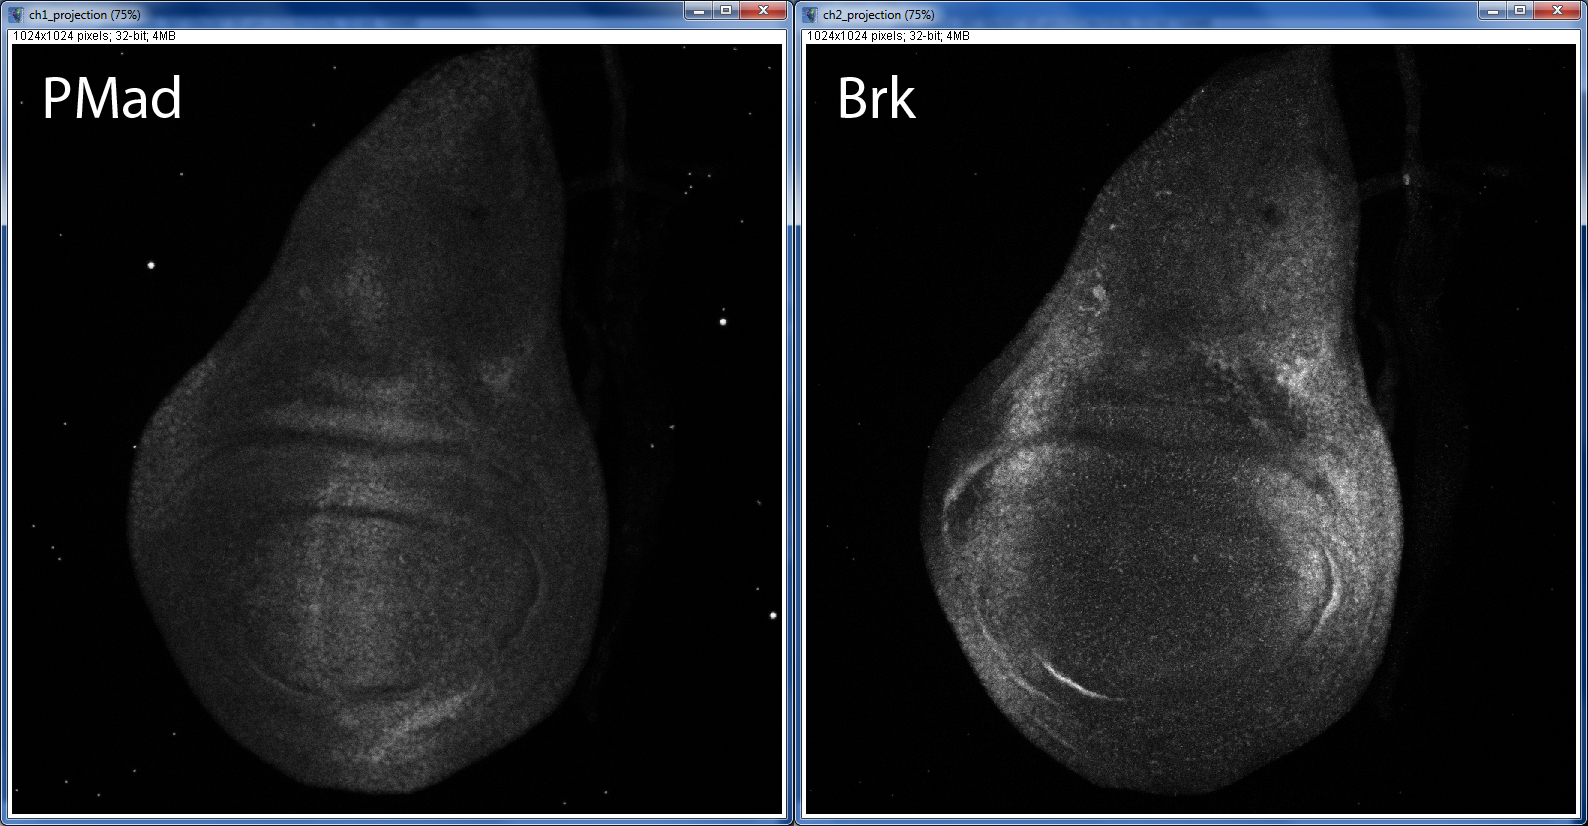
\includegraphics[scale=0.26]{images/wingj_expression_pmad_brk_projection.jpg}
\caption{\textbf{Mean intensity projections of Pmad-AB (Phosphorylated Mad) and Brk-AB (Brinker).} Antibodies (AB) are used to label their expression. Phosphorylated Mad (Pmad) is part of a complex that directly represses Brinker (Brk) \autocite{affolter2007decapentaplegic}. This is why the expressions of these two proteins are inversed.}
\label{fig:expression_pmad_brk_projection}
\end{figure}

% ===============================================================================
\section{Expression panel}
From the main interface of \wingj, click on \textit{Expression} to access the \textit{Expression panel}. \sectionref{fig:wingj_expression_interface} shows the options available for quantifying gene and protein expression levels from confocal fluorescence images. Actually, different options are proposed depending on the choice of the \textit{Type} of expression dataset to generate (\textit{Profiles} or \textit{Maps}). We give below a description of the main options that are common to both types of dataset. These options are included in the top section of the \textit{Expression panel} (\figref{fig:wingj_expression_interface}). The options relative to the generation of expression profiles and maps are later described in \sectionreftwo{sec:expression_profiles}{sec:expression_maps}, respectively.

\begin{figure}[!h]
\centering
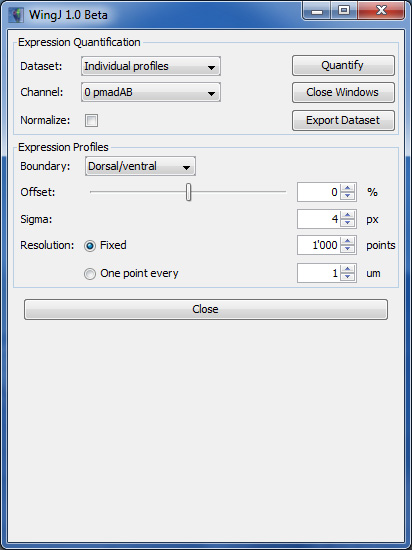
\includegraphics[scale=0.7]{images/expression_panel_1.jpg}
\caption{\textbf{Expression panel.} Click on \textit{Expression} from the main interface of \wingj to access tools for quantifying expression. The section on the top of the \textit{Expression panel} includes general options such as the selection of the channel to quantify, the type of expression dataset to generate (expression profiles or maps). The button \textit{Quantify} shows the output of the selected expression dataset and the button \textit{Export Dataset} exports the dataset to files.}
\label{fig:wingj_expression_interface}
\end{figure}

\begin{itemize}
 \item \textbf{Channel}. Defines the image channel to use as input for measuring expression.
 \item \textbf{Dataset}. If \textit{Individual profiles} is selected, expression will be measured along a trajectory included in the space of the structure model inferred (\sectionref{sec:expression_profiles}). If \textit{Individual maps} is selected, the expression information contained inside the entire space of the structure model is sampled to generate a \emph{scaleless} expression map (\sectionref{sec:expression_maps}). Select \textit{Reverse individual maps} to wrap an expression map on a given \wingj structure model (\sectionref{sec:expression_reversed_maps}). Finally, select \textit{Mean models} to integrate structure and expression models from multiple experiments to generate a robust quantitative description of the system considered (\sectionref{sec:community_expression_maps}).
 \item \textbf{Color}. Associates the color red (R), green (G) or blue (B) to the selected image channel. This option is used for generating composite images from one up to three channels (\sectionref{sec:expression_composite}). \textbf{Update: } This option is available when selecting the dataset \textit{Composite images}.
 \item \textbf{Normalize}. By default, expression is quantified from RGB 8-bit images (later converted to grayscale values) whose pixels take integer values between 0 (black) and 255 (white). If \textit{Normalize} is checked, the values measured are divided by 255 and so take floating point values in the range [0,1].
 \item \textbf{Quantify} (or \textbf{Generate}). Quantify expression. Depending on the selected \textit{Dataset} (\textit{Individual profiles} or \textit{Individual maps}), the output shown will be different as described in \sectionreftwo{sec:expression_profiles}{sec:expression_maps}. If \textit{Dataset} is set to \textit{Reverse individual map} or \textit{Mean models}, this button will become a \textit{Generate} button.
 \item \textbf{Close Windows}. Closes all the windows previously opened by the button \textit{Quantify} or \textit{Generate}.
 \item \textbf{Composite}. Generates a RGB composite image from the opened image channels. Use the option \textit{Color} to assign a color to each image channel. Up to three channels can be used in the initial release of \wingj for generating composite images. Takes into account the index of the minimum and maximum z-slice and projection method specified for each channel from the main interface of \wingj. \textbf{Update: } This option is available when selecting the dataset \textit{Composite images}.
 \item \textbf{Export Dataset}. Opens a \textit{Save} dialog to export expression dataset. The filename entered (without extension) is used as a prefix to name multiple files. The content of the dataset depends on \emph{Dataset} as explained in \sectionreftwo{sec:expression_profiles_dataset}{sec:expression_maps_dataset}.
\end{itemize}

\textbf{Important}: Normalizing expression profiles divides every measurement by 255 and NOT by the maximum value obtained from a given profile. Thus, normalized expression profiles or maps obtained for different experiments can still be compared.

% ===============================================================================
\section{Generating individual expression profiles}\label{sec:expression_profiles}
\subsection{Overview}
Start by specifying which channel you want to quantify, select \textit{Individual profiles} and click on \textit{Quantify}.\\

\wingj will first display the trajectory along which expression is measured as shown in \figureref{fig:wingj_expression_profiles_preview}. The second window shows the expression levels measured along this trajectory. The options \textit{Boundary} and \textit{Offset} can be set to define a new trajectory inside the structure model identified.\\

In \figureref{fig:wingj_expression_profiles_preview}, expression is measured along the D/V compartment boundary from the anterior to posterior side. Right-clicking on the profile window will display a menu which provides additional options.\\

\begin{figure}[!h]
\centering
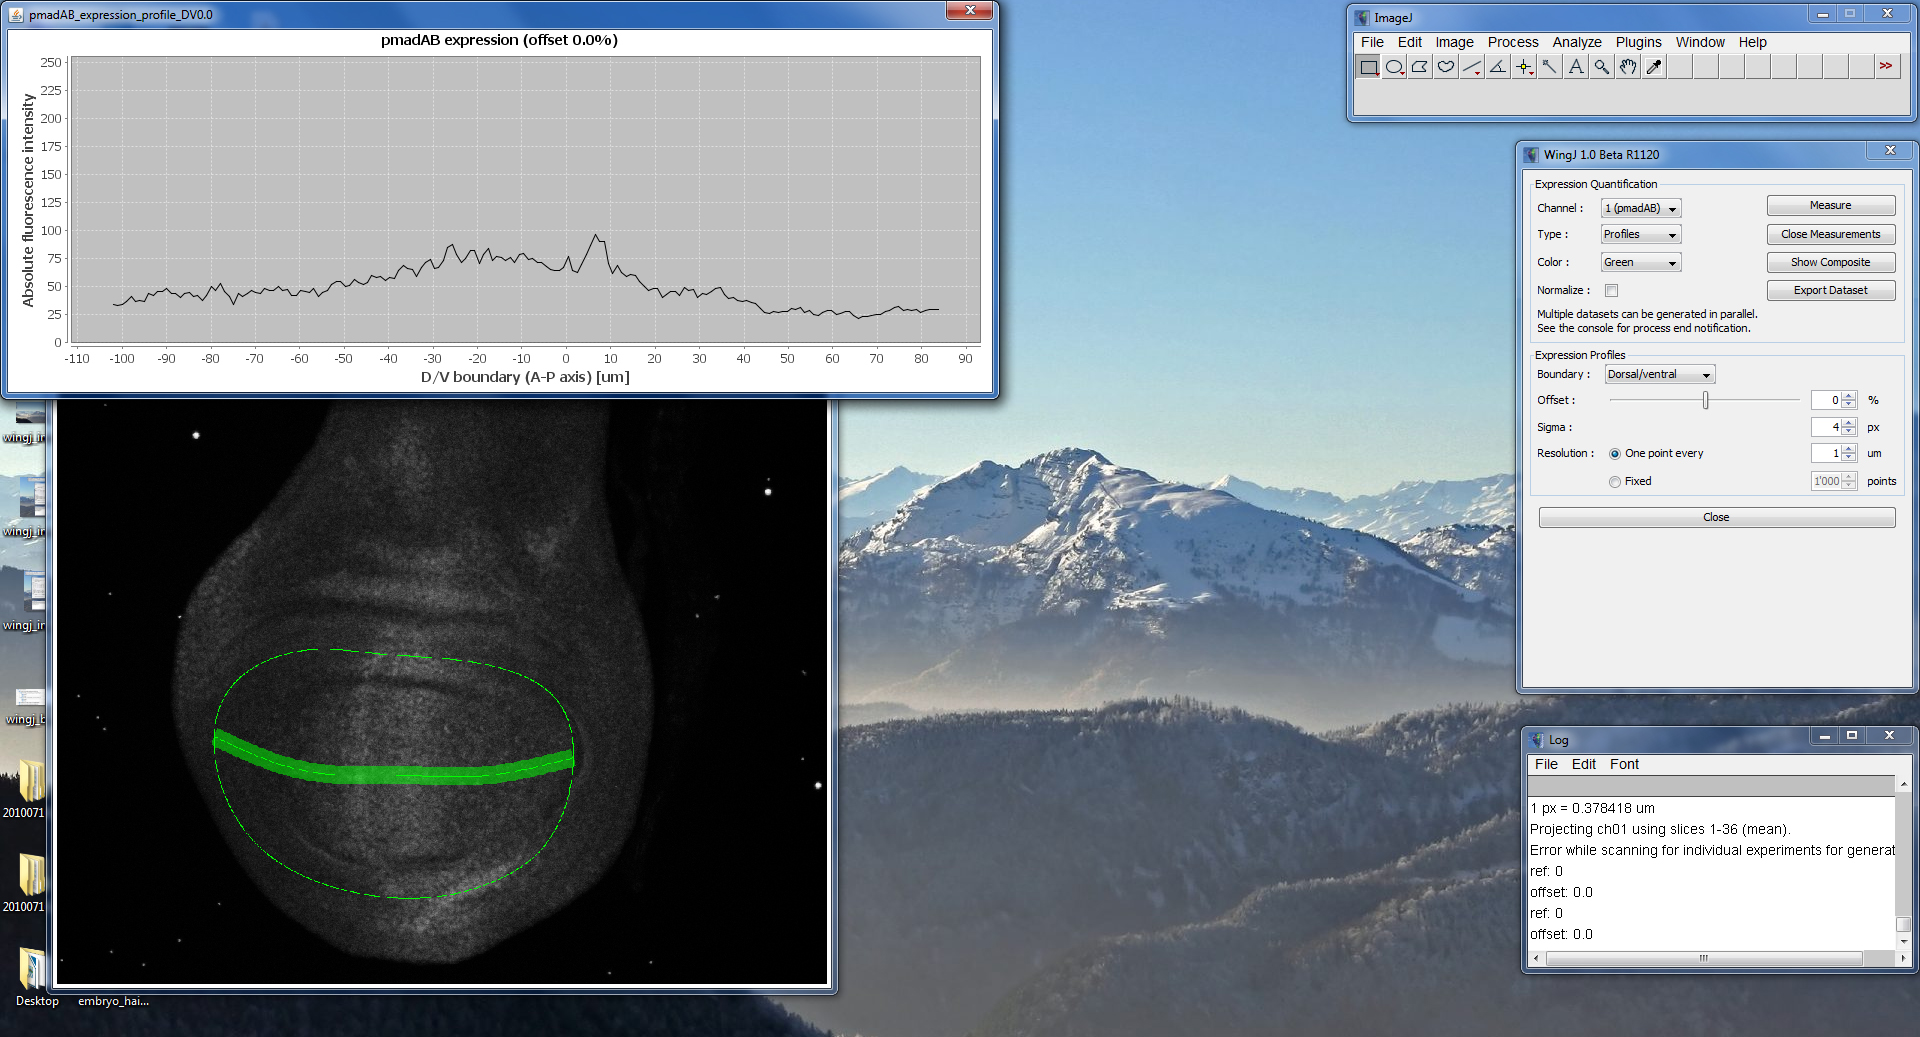
\includegraphics[scale=0.215]{images/wingj_expression_profiles_preview.jpg}
\caption{\textbf{Illustration of the content of the expression dataset \textit{Individual profiles} generated for Pmad.} First, a window shows where expression is measured (here along the D/V boundary) inside the structure model identified in \sectionref{chap:structure}. A second window reports the expression profile obtained by measuring expression along the given trajectory. Click on \textit{Export Dataset} to save the preview of the trajectory in TIFF format, and the expression profile both in PDF and text format (\sectionref{sec:expression_profiles_dataset}).}
\label{fig:wingj_expression_profiles_preview}
\end{figure}

An example is given in \sectionref{sec:matlab_profiles} where many expression profiles are combined together using the \wingjMatlab to obtain representative expression profiles as shown in \sectionref{fig:wingj_expression_profiles_demo}. Such expression profiles are particularly suitable for studying scaling \autocite{de2010precision,hamaratoglu2011dpp} or reverse engineering gene networks \autocite{jaeger2004dynamic,perkins2006reverse}, for instance.\\

\begin{figure}[!h]
\centering
% 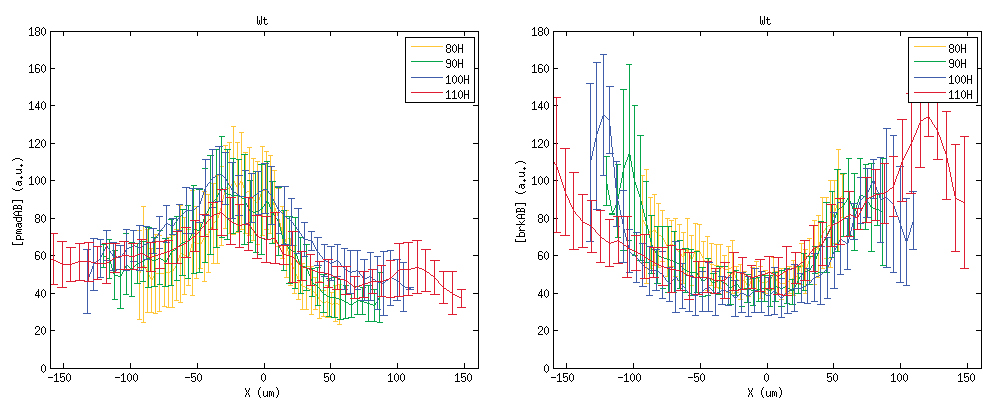
\includegraphics[scale=0.4]{images/wingj_expression_profiles_demo.jpg}
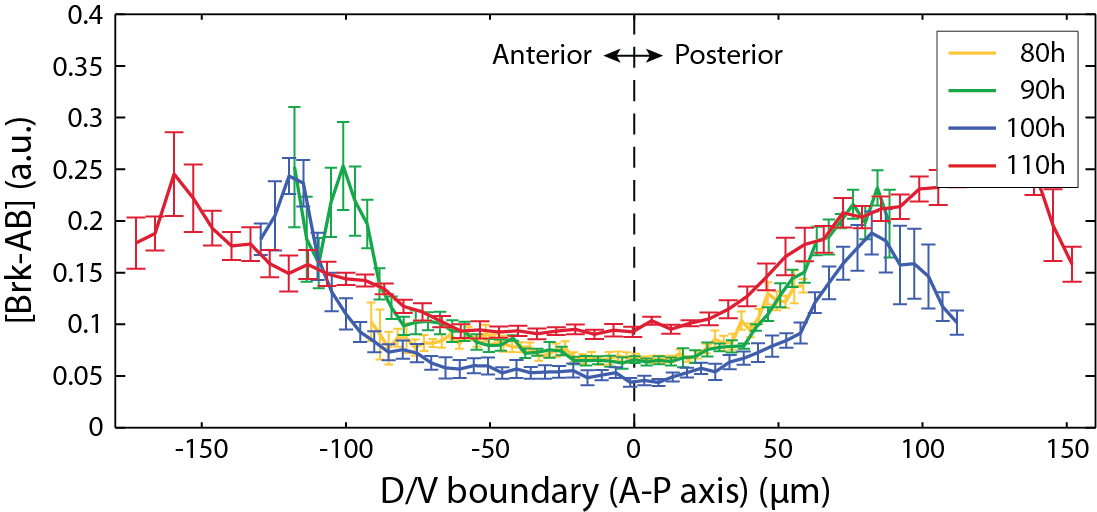
\includegraphics[scale=1]{images/brkAB_profile_for_user_manual.jpg}
\caption{\textbf{Example of the integration of many expression profiles using the \wingjMatlab.} The expression profiles generated by \wingj for many experiments (e.g. many wings) can be combined to obtain more representative profiles. Here the expression of Brk is measured along the D/V compartment boundary in 80h-, 90h-, 100h- and 110h-old wild type wings. For each type or class of experiments (here for different time points), five to ten wings are quantified using \wingj before integrating the individual expression profiles using the \wingjMatlab to compute the mean and standard error at different points along the selected trajectory (\sectionref{sec:matlab_profiles}).}
\label{fig:wingj_expression_profiles_demo}
\end{figure}

\textbf{Important}: Note the following convention about the $x$-axis of the expression profiles: the origin corresponds to the intersection of the trajectory with the A/P or D/V boundary, depending on the choice of the reference boundary. Negative $x$ values always correspond to the anterior or ventral side of the structure and positive values to the posterior or dorsal side.

% ===============================================================================
\subsection{Options}
The options displayed below are available when \textit{Dataset} is set to \textit{Individual profiles} (\figref{fig:wingj_expression_profiles_interface}):

\begin{figure}[!h]
\centering
% 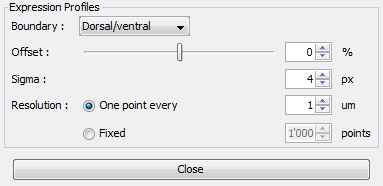
\includegraphics[scale=0.7]{images/wingj_expression_profiles_interface_crop.jpg}
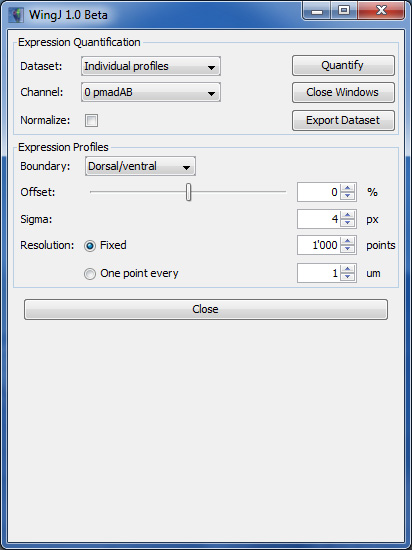
\includegraphics[scale=0.7]{images/expression_panel_1.jpg}
\caption{\textbf{Options for generating expression profiles.} These options are available in the \textit{Expression panel} when \textit{Dataset} is set to \textit{Individual profiles}.}
\label{fig:wingj_expression_profiles_interface}
\end{figure}

\begin{itemize}
 \item \textbf{Boundary}. The \textit{reference boundary} is the A/P or D/V compartment boundary. This boundary is used as a reference to compute the trajectory along which expression will be measured.
 \item \textbf{Offset}. Takes a value between -100\% and 100\%. If set to 0, expression is measured along the selected reference boundary.
    \begin{itemize}
     \item \textit{D/V is the reference boundary}: negative/positive offsets generate versions of the D/V boundary translated along the A/P boundary towards the ventral/dorsal side (\figrefsub{fig:wingj_expression_profiles_trajectories}{A}).
     \item \textit{A/P is the reference boundary}: negative/positive offsets generate versions of the A/P boundary translated along the D/V boundary towards the anterior/posterior side (\figrefsub{fig:wingj_expression_profiles_trajectories}{B}).
    \end{itemize}
 \item \textbf{Sigma}. Standard deviation $\sigma$ of the 1D Gaussian filter built perpendicularly to the trajectory along which expression is measured. Click on \textit{Measure} to get a preview of where this trajectory is located in the space of the structure model. The width of the measurement domain is $6\sigma$. Larger values of $\sigma$ make this domain wider and so smooth the expression profile.
 \item \textbf{Resolution}. Defines the number of measurement points along the measurement trajectory.
    \begin{itemize}
     \item \textit{Fixed} is selected: defines precisely the number of measurement points.
     \item \textit{One point every} is selected: sets the distance between two measurement points (e.g. in \mum, the unit is set depending on the meta-information found in the input images).
    \end{itemize}
\end{itemize}

\figureref{fig:wingj_expression_profiles_trajectories} shows the result of different combinations of the parameter \textit{Boundary} and \textit{Offset}. Please remember the convention that is to measure expression from anterior to posterior side and from ventral to dorsal side. This convention comes from our definition of the \emph{canonical orientation} as stated in the \textbf{Supplementary Notes} of our paper\autocite{schaffter2013}.

\begin{figure}[!h]
\centering
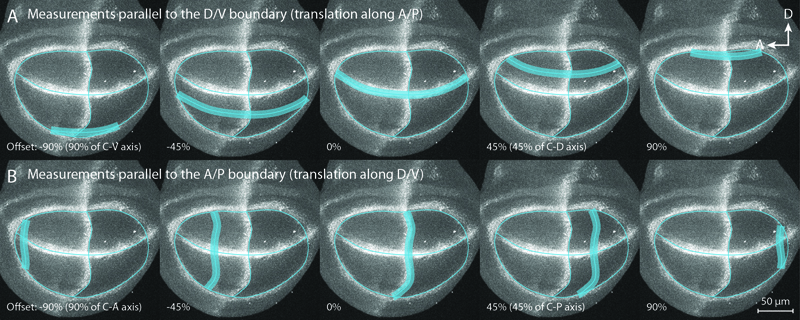
\includegraphics[scale=0.52]{images/wingj_expression_profiles_trajectory.jpg}
\caption{\textbf{Illustration of the effect of the parameter \textit{Boundary} and \textit{Offset} for defining expression measurement trajectories.} Translated versions of the A/P and D/V compartment boundaries are automatically cropped to only consider expression inside the identified structure model.}
\label{fig:wingj_expression_profiles_trajectories}
\end{figure}

% ===============================================================================
\subsection{Dataset}\label{sec:expression_profiles_dataset}
Click on \textit{Quantify} to generate and visualize the expression dataset. Click on \textit{Close Windows} to close all the windows opened so far by clicking on \textit{Quantify}. To visualize the effect of a parameter (e.g. \textit{Offset}), change its value and click again on \textit{Quantify} to show the updated expression dataset.\\

You can then click on \textit{Export Dataset} to write the dataset to files. We strongly recommend to keep as often as possible the default filename sugggested by \wingj because the proposed filenames satisfy a naming convention used by the \wingjMatlab (\sectionref{chap:matlab}). Then click on \textit{Save} to write the dataset to files. An example of the content of an expression profile dataset generated for Pmad is given below:

\begin{itemize}
 \item \textbf{pmadAB\_expression\_profile\_DV-50.0.pdf}. PDF document containing the expression profile. The default filename contains the following information:
    \begin{itemize}
     \item \textit{pmadAB}: name of the gene or protein whose expression has been measured.
     \item \textit{expression\_profile}: identifies the dataset as expression profile.
     \item \textit{DV}: the reference boundary is D/V.
     \item \textit{-50}: offet is set to -50. This means that the trajectory initially parallel to the D/V compartment boundary is translated along 50\% of the A/P boundary to the anterior direction (positive offsets would have resulted in a translation to the posterior direction).
    \end{itemize}
 \item \textbf{pmadAB\_expression\_profile\_DV-50.0.txt}. Text file in TSV format (tab separated values) containing the raw data of the expression profile. This file is used by the \wingjMatlab to plot expression profiles. The first two columns contain the $x$-axis (e.g. in \mum) and $y$-axis ([0,255] or [0,1] if \textit{Normalize} is checked) of the profile. The third and fourth columns contain the coordinates of the points of the trajectory in the image space of the image (in \px).
 \item \textbf{pmadAB\_expression\_profile\_DV-50.0.tif}. TIFF image that shows where the expression has been measured (content of the preview window displayed when clicking on \textit{Quantify} as shown in \figref{fig:wingj_expression_profiles_trajectories}).
\end{itemize}

% ===============================================================================
\section{Generating individual expression maps}\label{sec:expression_maps}
% ===============================================================================
\subsection{Overview}
Set \textit{Dataset} to \textit{Individual maps} to reveal new options in the \emph{Expression panel} for generating \textit{expression maps}.\\

Expression maps provide a convenient representation for integrating expression maps obtained from many individual experiments. To build such maps, we took inspiration from the parametrization of the surface of Earth to define a grid coordinate system based on the parametric structure model identified \autocite{schaffter2013}. The nodes of the grid indicate where expression is sampled before building a \emph{scaleless} disc-shape expression map. There are actually two different expression maps which can be generated depending on which boundary (A/P or D/V) is selected as the equator of the grid coordinate system (\figref{fig:expression_grids}). Expression along the equators will be preserved while locations far away from it are affected by distortions due to oversampling in those remote regions. \figureref{fig:wingj_expression_maps_preview} shows the two expression maps obtained for Pmad when selecting the boundary A/P (left) and D/V (right) as equator. Here setting the equator along the A/P boundary leads to less visible distortions because Pmad is mainly expressed along this boundary.\\

\begin{figure}[!h]
\centering
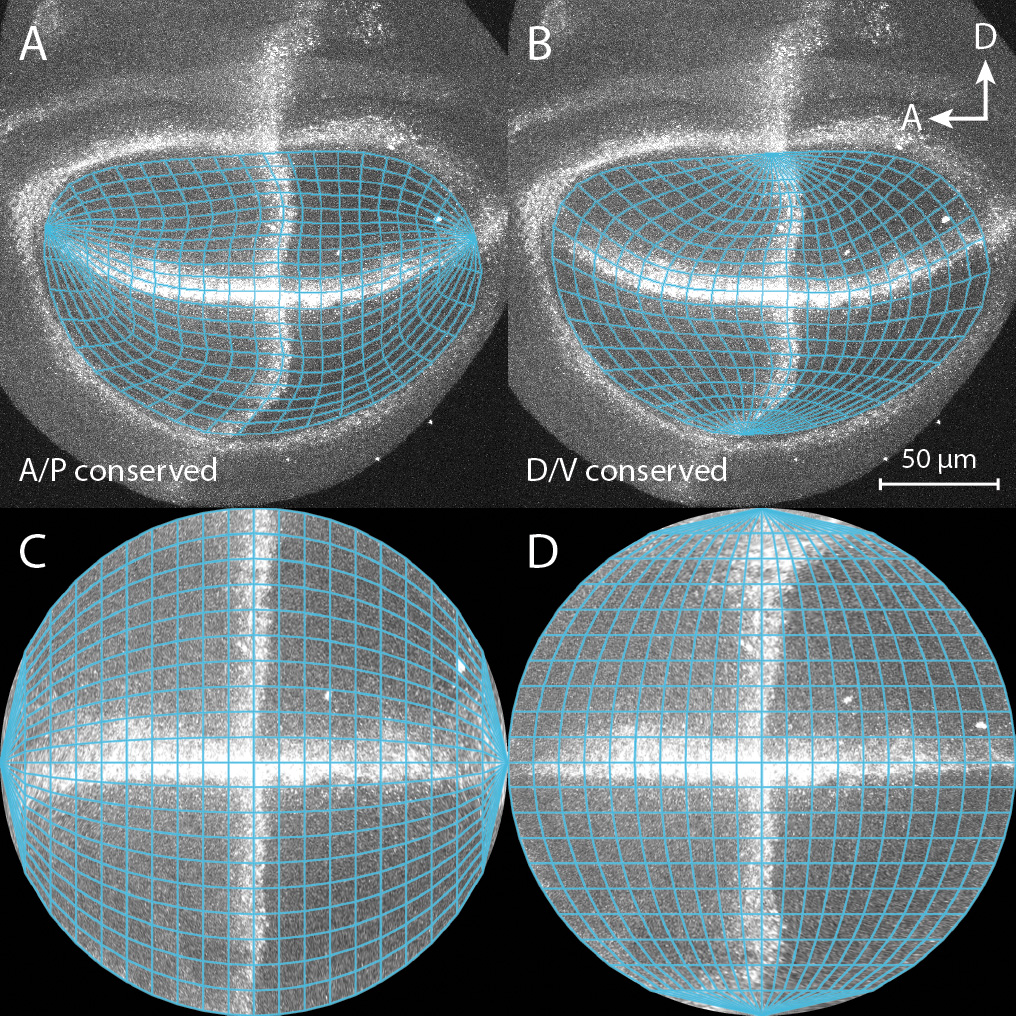
\includegraphics[scale=0.3]{images/expression_grids.jpg}
\caption{\textbf{Parametric grids for quantifying expression in the \droso wing.} The parametric model of wing pouch structure identified in \sectionref{chap:structure} is derived to build a grid inspired from the parametrization of the surface of Earth and whose intersections indicate where expression measurements should be sampled. Two different grids are obtained depending on the choice of the \emph{equator} (A/P or D/V compartment boundary). (A-B) The equator of the grid is set along the A/P and D/V boundary, respectively. (C-D) By looking at the expression of Wg-Ptc, we observe that its expression is mainly conserved along the A/P and D/V boundary, respectively. For visualization purpose, the density of the grid here is one thousand times less than the effective measurement grids.}
\label{fig:expression_grids}
\end{figure}

\begin{figure}[!h]
\centering
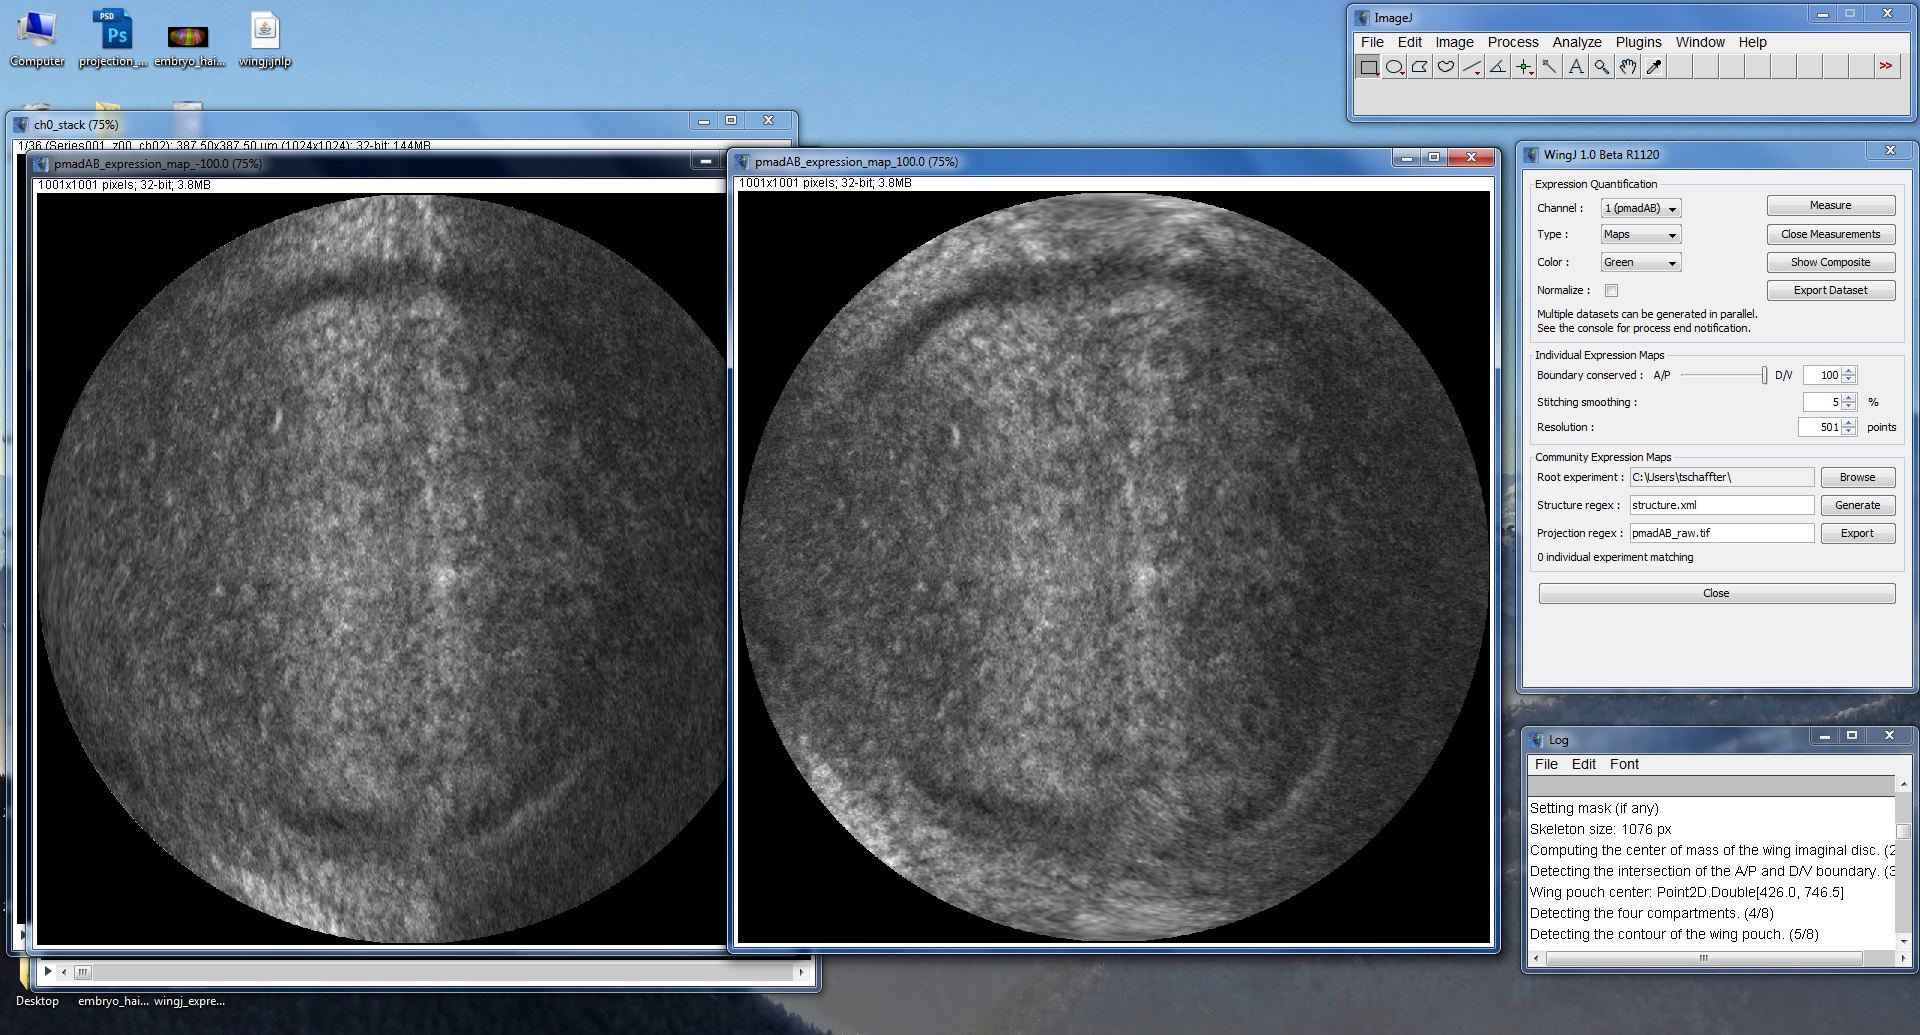
\includegraphics[scale=0.215]{images/wingj_expression_maps_preview.jpg}
\caption{\textbf{Generation of two different expression maps for Pmad depending on the choice of the equator for defining the sampling grid.} The expression maps on the left and right are obtained when setting the equator of the sampling grid to A/P (\textit{Boundary conserved} is set to -100\%) and D/V (\textit{Boundary conserved} is set to 100\%), respectively. Here, setting the equator along the A/P boundary leads to less visible distortions because Pmad is mainly expressed along this boundary. If the value of the slider \textit{Boundary conserved} is set to 0, a different expression map will be created from stitching the two previous maps in order to have expression conserved along both the A/P and D/V boundaries. However, this may introduce discontinuities where the two original maps, where A/P and D/V are fully conserved, are stitched together. The parameter \textit{Stitching smoothing} can be used to make the stitching boundary less visible. If \textit{Boundary conserved} takes values in [-100\%,0\%[, conserving the A/P boundary will be more important than conserving the D/V boundary, and the other way around when using values in ]0\%,100\%]. Click on \textit{Export Dataset} to save the expression map and its binary mask in TIFF formats, as well as the input image projection used to generate the expression map and its binary mask, which has the shape of the structure model inferred.}
\label{fig:wingj_expression_maps_preview}
\end{figure}

One of the main features of the individual expression maps is that their geometry is independent of the shape of the structure models. Therefore they provide a convenient representation for integrating expression data from multiple experiments. For instance, a \textit{mean} or \textit{standard deviation} expression map can be easily computed. Moreover, expression maps enable to compare directly gene and protein expression between wild type and mutant experiments, for instance. Yet another benefit is that expression maps allow to compare the expression of a given gene or protein in wings imaged at two different time points, e.g. to compare the domain of expression of Pmad at 80 and 90 hours AEL. This is illustrated in \figureref{fig:wingj_expression_maps_circular_demo}, which has been generated using the \wingjMatlab (\sectionref{chap:matlab}). The figure reports the difference in expression of five genes between wild type and \textit{pent} deficient wings (\textit{pent$^{2-5}$} - wild type) for different time points \autocite{schaffter2013}. For example, we observe clearly that the expression of Pmad at 100 hours is restrained in the center of the pouch in \textit{pent$^{2-5}$} experiments as it has been previously observed in individual wings \autocite{hamaratoglu2011dpp}. Each mean circular expression map shown in \figureref{fig:wingj_expression_maps_circular_demo} has been computed by averaging the individual expression maps of ten to twenty wings.\\

\begin{figure}[!h]
\centering
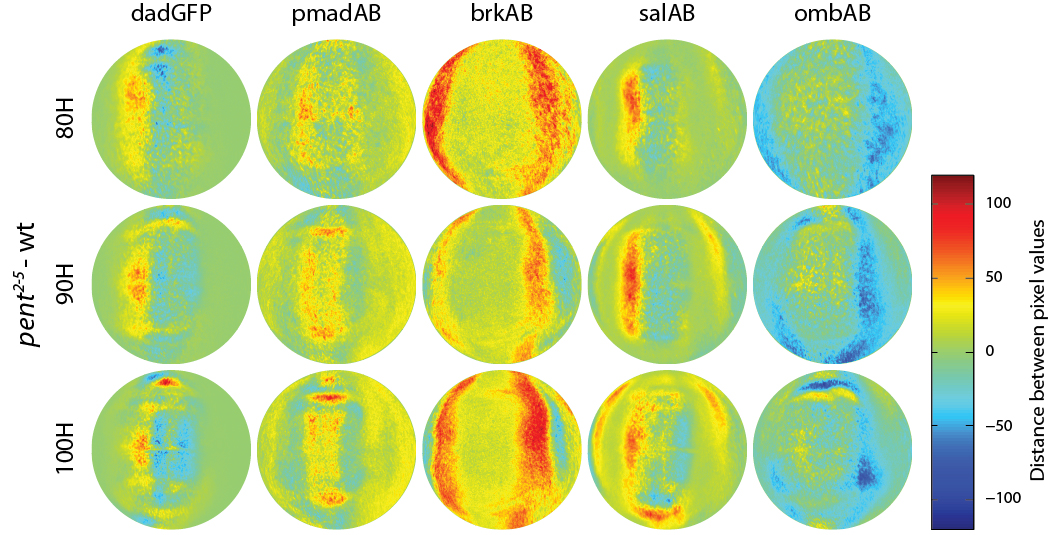
\includegraphics[scale=0.4]{images/wingj_expression_maps_circular_demo.jpg}
\caption{\textbf{Generation of mean \textit{scaleless} expression maps using the \wingjMatlab.} First, five to ten wings have been quantified using \wingj to generate individual, circular expression maps (equator set to the A/P boundary) for wild type and \textit{pent$^{2-5}$} wings and for 80-, 90-, and 100-hour-old wings. For each type of experiments, the mean circular expression map is computed and the difference between wild type and \textit{pent$^{2-5}$} mutation maps is reported (\textit{pent$^{2-5}$} - wild type). A color above green (i.e. pixels distance above zero) means that a given protein is more expressed at a given location in \textit{pent$^{2-5}$} than in wild type wings. For instance, we observe that the expression of Pmad is more constrained to the center of the wing pouch in \textit{pent$^{2-5}$} than in wild type wings. This is consistent with previous observations \autocite{hamaratoglu2011dpp}.}
\label{fig:wingj_expression_maps_circular_demo}
\end{figure}

\textbf{Important:} Actually, we mainly use the mean circular expression maps as an intermediate representation for generating more detailed models of biological systems (\sectionref{sec:community_expression_maps}).

% ===============================================================================
\subsection{Options}
Setting \textit{Dataset} to \textit{Individual maps} displays two option boxes in the \textit{Expression panel}. The first box is shown in \figureref{fig:wingj_expression_maps_circular_interface} and provides options to generate individual circular expression maps.

\begin{figure}[!h]
\centering
% 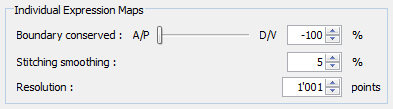
\includegraphics[scale=0.7]{images/wingj_expression_maps_circular_interface_crop.jpg}
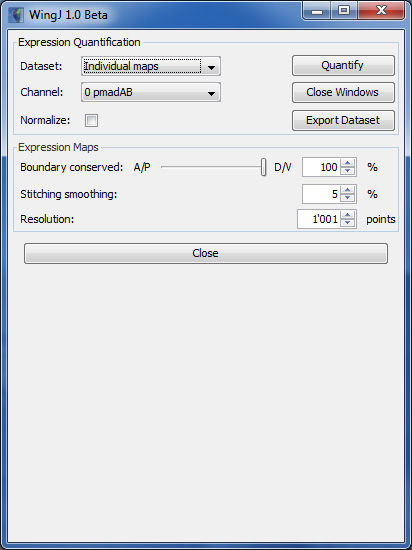
\includegraphics[scale=0.7]{images/expression_panel_2.jpg}
\caption{\textbf{Options for generating individual expression maps.} These options are available in the \textit{Expression panel} when \textit{Dataset} is set to \textit{Individual maps}.}
\label{fig:wingj_expression_maps_circular_interface}
\end{figure}

% More importantly, consider exporting one of the these two circular expression maps (set \textit{Boundary conserved} to either -100 or 100) as we propose in the next section a method to 1) combine multiple circular expression maps sampled from different wing pouches and 2) wrap the combined, circular expression map obtain on a structure whose shape is similar to the one of a wing pouch (Section XXX).\\

Click on \textit{Quantify} to generate and visualize the expression map. The options available for generating expression maps are:

\begin{itemize}
 \item \textbf{Boundary conserved}. Places the grid equator along the A/P boundary if set to -100\%, and places the grid equator along the D/V boundary if set to 100\%. Intermediate values allow to combine the two types of circular expression maps: negative values allow to better conserve the expression along the A/P than the D/V boundary, while positive values promote the conservation of the expression along the D/V boundary.
 \item \textbf{Stitching smoothing}: Provides control over the stitching of the two original circular expression maps when the parameter \textit{Boundary conserved} is set to a value different than -100\% and 100\%.
 \item \textbf{Resolution}. Defines the dimension in \px of the expression map (the circular map is included in a square image).
\end{itemize}

% ===============================================================================
\subsection{Dataset}\label{sec:expression_maps_dataset}
Click on \textit{Export Dataset} to save the dataset. The files written are:

\begin{itemize}
 \item \textbf{dadGFP\_expression\_map.tif}. circular expression map embedded in a square image in TIFF format.
% The token \textit{-100} tells that the dataset has been generated using \textit{Boundary conserved} set to -100, i.e. where the expression along the A/P boundary is conserved.
 \item \textbf{dadGFP\_expression\_map\_mask.tif}. Binary image in TIFF and square format that can be used as a mask. Pixels corresponding to the circular expression map are set to white (255), otherwise black (0). That is, the mask is a black square image with a white disc centered on the image and whose diameter is equal to the width of the image).
%  \item \textbf{dadGFP\_expression\_map\_raw.tif}. Projection of the image stack used to generete the circular expression map.
%  \item \textbf{dadGFP\_expression\_map\_raw\_mask.tif}. Binary image in TIFF format that can be used as a mask. Pixels falling inside the structure model are set to white, otherwise black.
\end{itemize}

% ===============================================================================
\section{Reversing individual expression maps}\label{sec:expression_reversed_maps}
Set \textit{Dataset} to \textit{Reverse individual maps} provides options to wrap an expression map on \textit{any} structure models generated and exported to file using \wingj (\figref{fig:wingj_expression_maps_circular_interface_reversed}). First, select a file describing a \wingj structure model. You can also decide to use the structure model active in \wingj, which can be visualized and edit via the \textit{Structure panel} accessible from the main interface. Then, select the circular expression map (image file) to reverse and specify if the A/P or D/V boundary has been used at the time of generating this expression map (see the description of the parameter \textit{Boundary conserved} in \sectionref{sec:expression_profiles}). Finally, click on \textit{Quantify} to visualize the result or click on \textit{Export Dataset} to directly save it to file.

\begin{figure}[!h]
\centering
% 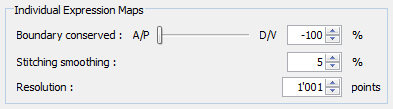
\includegraphics[scale=0.7]{images/wingj_expression_maps_circular_interface_crop.jpg}
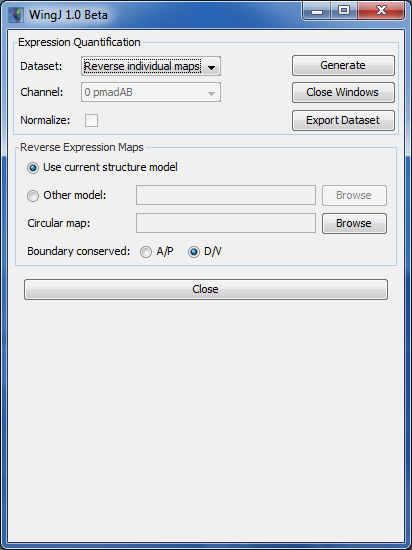
\includegraphics[scale=0.7]{images/expression_panel_3.jpg}
\caption{\textbf{Options for wrapping individual circular expression maps on structure models.} These options are available in the \textit{Expression panel} when \textit{Dataset} is set to \textit{Reverse individual maps}.}
\label{fig:wingj_expression_maps_circular_interface_reversed}
\end{figure}

% ===============================================================================
\section{Generating mean structure and expression models}\label{sec:community_expression_maps}
% ===============================================================================
\subsection{Overview}
The circular expression map representation we developed and introduced in \sectionref{sec:expression_maps} is very important as it allows the integration of 2D expression data from multiple wings, embryos or any other organ or body systems. Note that the same approach could be extended to a 3D expression representation if the structure model inferred is also in three spatial dimensions.\\

Here, we introduce an additional mechanism we developed to wrap a \textit{mean circular expression map} on a \textit{mean structure model}. Here, the circular expression map is used as an intermediate state required for data integration before giving it the shape of a wing pouch structure, for instance. We call this last representation \textit{structure and expression mean model} or simply \textit{mean model} as it includes information from many experiments.\\

Set \textit{Dataset} to \textit{Mean models}. The options to generate mean models are displayed in the last box of the \textit{Expression panel}. The requirements for each experiment are a \wingj structure model file and a projection of the stack of confocal fluorescence images to quantify. Individual expression maps will then be automatically computed by \wingj before generating and displaying the obtained mean model (\figref{fig:wingj_expression_agg_demo}). In the next section, we describe in more details how to generate mean models from individual experiments.\\

\begin{figure}[!h]
\centering
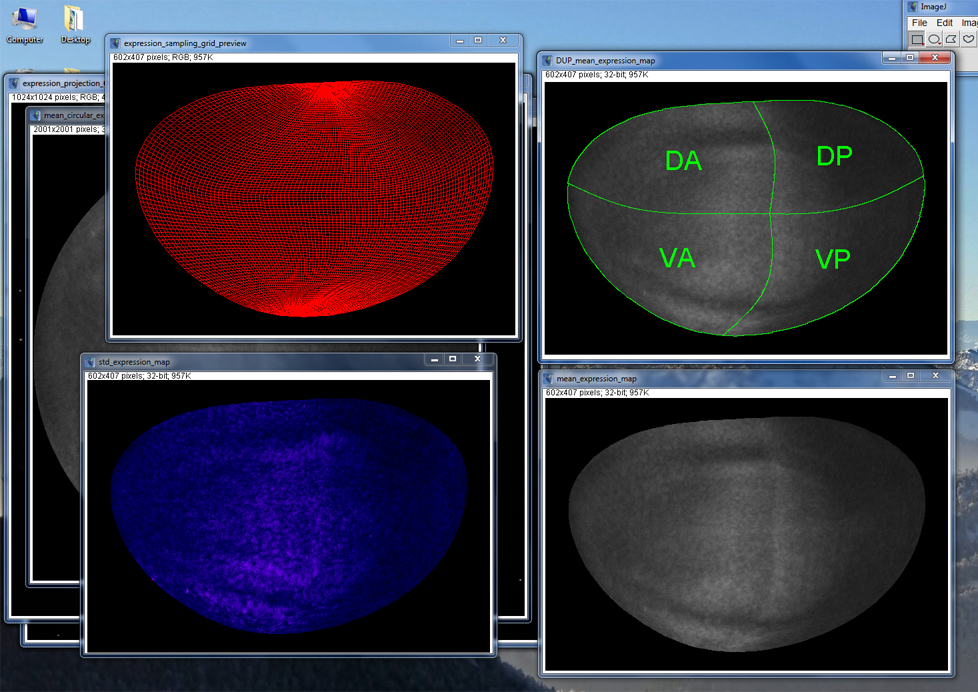
\includegraphics[scale=0.42]{images/expression_agg_demo_720p_crop.jpg}
\caption{\textbf{Generation of a structure and expression aggregated model or \textit{mean model} including information about the structures and expression of many experiments.} The method requires for each experiment that the structure of the system has been previously quantified using \wingj and exported to files. Idem for the input image projection that will be directly used to measure expression (click on the button \textit{Save} from the main interface to compute and export the projections of the loaded image stacks). During the aggregation process, the structures of the experiments are averaged to produce a robust quantitative description of the structure. Two additional structures are saved. They correspond to the average structure $\pm$ the standard deviation (only visible when the dataset is exported to files). Then, individual expression maps are generated for each experiment before averaging them and wrapping the output on the mean structure model. (Top-left) Mean structure model. The grid defines how expression is sampled (the grid shown is a down-sampled version of the real grid). (Top-right) Mean model augmented with the location of the A/P and D/V compartment boundaries. The orientation of the model is also shown. Note that the orientation of the mean models are always set to the canonical orientation (anterior is left and dorsal is top). (Bottom) Mean and standard deviation of the expression data computed from many experiments, here on the right and left, respectively. Here, the \ij colormap \textit{Fire} is used for the standard deviation expression map and can be changed through the menu \textit{Image} $>$ \textit{Lookup Tables}.}
\label{fig:wingj_expression_agg_demo}
\end{figure}

% ===============================================================================
\subsection{Options}
Click on \textit{Browse} from the \textit{Expression panel} to select the \textit{experiments root directory} (\sectionref{sec:root_directory}) which contains the individual experiment folders. As described in \sectionref{sec:experiment_directory}, each experiment folder must contain two sub-folders called \textit{images} (contains the stacks of confocal images) and \textit{WingJ} (where datasets are exported from \wingj). This \textit{signature} is used to identify the experiment folders contained in the selected experiments root directory.\\

Once again, the generation of a mean models requires for each experiment a \wingj structure model file and the image projection of the gene or protein to quantify previously saved in TIFF format (\figref{fig:wingj_expression_maps_mean_interface}), for instance by clicking on the button \emph{Save}. These two files must have been saved in the sub-folder \textit{WingJ}. In order to select multiple files at the same time and for flexibility purpose, two \textit{regular expression (regex)} can be specified in \textit{Structure regex} (to select the \wingj structure model files) and \textit{Projection regex} (to select the image projection of the gene or protein to quantify previously saved in TIFF format). Finally, click on \textit{Generate} to compute and display the mean expression map, or click on \textit{Export} to save it in TIFF format along with the target structure model and a binary mask in TIFF format.

% Then, select the target structure model on which the mean circular expression map will be wrapped on (see options below)

\begin{figure}[!h]
\centering
% \includegraphics[scale=0.7]{images/wingj_expression_maps_mean_interface.jpg}
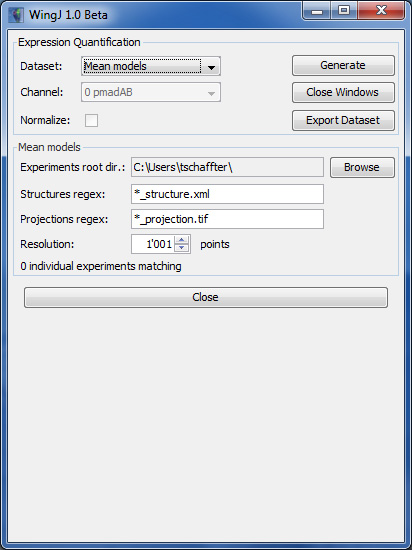
\includegraphics[scale=0.7]{images/expression_panel_4.jpg}
\caption{\textbf{Options for generating mean models.} These options are available in the \textit{Expression panel} when \textit{Dataset} is set to \textit{Mean models}.}
\label{fig:wingj_expression_maps_mean_interface}
\end{figure}

\begin{itemize}
 \item \textbf{Experiments root experiment}. Path to the \textit{experiments root directory} (\sectionref{sec:root_directory}) which contains the individual experiment folders.
 \item \textbf{Structure regex}. Regular expression to select the structure model files from each experiment folder. To give an example, let's suppose that the sub-folder \textit{WingJ} included in each experiment folder contains, for some reasons, two structure model files named \textit{structure.xml} and \textit{structure\_EXP.xml} where \textit{EXP} is a string different for each file, for instance the name and/or index of the experiment. We describe three scenarios to illustrate the use of the regular expressions:
    \begin{itemize}
     \item \textit{Structure regex contains ``structure.xml''}: the file \textit{structure.xml} is selected without ambiguities for each experiment.
     \item \textit{Structure regex contains ``structure\_*.xml''}: the second type of structure model files is selected even if they have different filenames. This is achieved by using the char '*' which is called \textit{wildcard}.
     \item \textit{Structure regex contains ``structure*.xml}: here it's an ambiguous case because \textit{structure.xml} and \textit{structure\_EXP.xml} satisfy both the given regex. Whenever there is an ambiguity for an experiment folder, \wingj discards it from the set of experiments to use for generating the mean expression map. The number of ambiguous cases is reported by \wingj in the graphical user interface.
    \end{itemize}
 \item \textbf{Projection regex}. Regular expression to select the image projection files in TIFF format from each experiment folder. This regex works the same way as the structure regex.
%  \item \textbf{Target structure}. Specifies how the target structure is generated or selected (see below). The mean circular expression map computed will then be wrapped on the target structure model. There are three ways to define the target structure model.
%     \begin{itemize}
%      \item \textit{Synthetic}: generates a \textit{mean} structure model from the individual structure models provided.
%      \item \textit{Area-based}: computes the mean area of the structure model and pick the one whose area is the closest to the mean area.
%      \item \textit{Manually}: requires the user to give the index of an experiment whose structure model will be used as target structure model. Since it is not straight forward in which order \wingj lists the experiments, please refer to the \textit{Log window} to know which index corresponds to which experiment.
%     \end{itemize}
\end{itemize}


\begin{figure}[!h]
\centering
% \includegraphics[scale=0.7]{images/wingj_expression_maps_mean_interface.jpg}
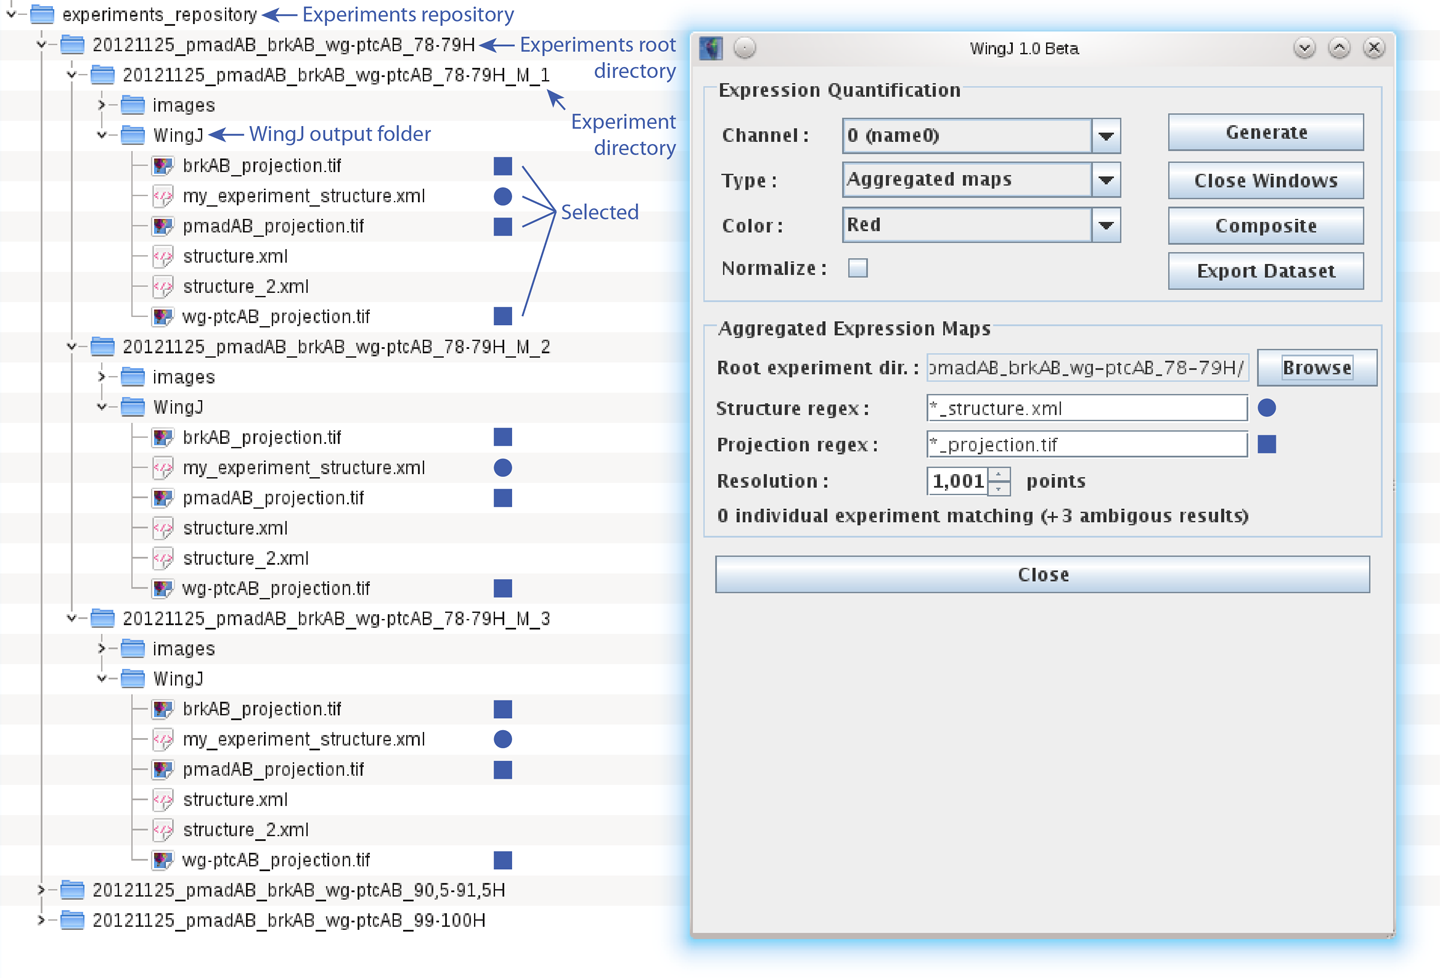
\includegraphics[scale=1.2]{images/regex1_cropped_1440.png}
\caption{\textbf{Selection of individual structure and expression models using regular expressions.} One structure model and one gene or protein expression projection must be selected for each experiment. Regular expressions (regex) provide a convenient way to easily select the files from each experiment directory. Enter a string in the structure and projection fields to identify the files. The wildcard '*' can be used to match any substring, even empty strings. Here, \wingj notifies that it found three ambiguous results because the image projection is not uniquely identified. If \wingj finds clear results and ambiguous results, only the clear results will be integrated to generate the mean model. Note that the name of the \wingj output folder must be called "WingJ".}
\label{fig:wingj_regex1}
\end{figure}

\begin{figure}[!h]
\centering
% \includegraphics[scale=0.7]{images/wingj_expression_maps_mean_interface.jpg}
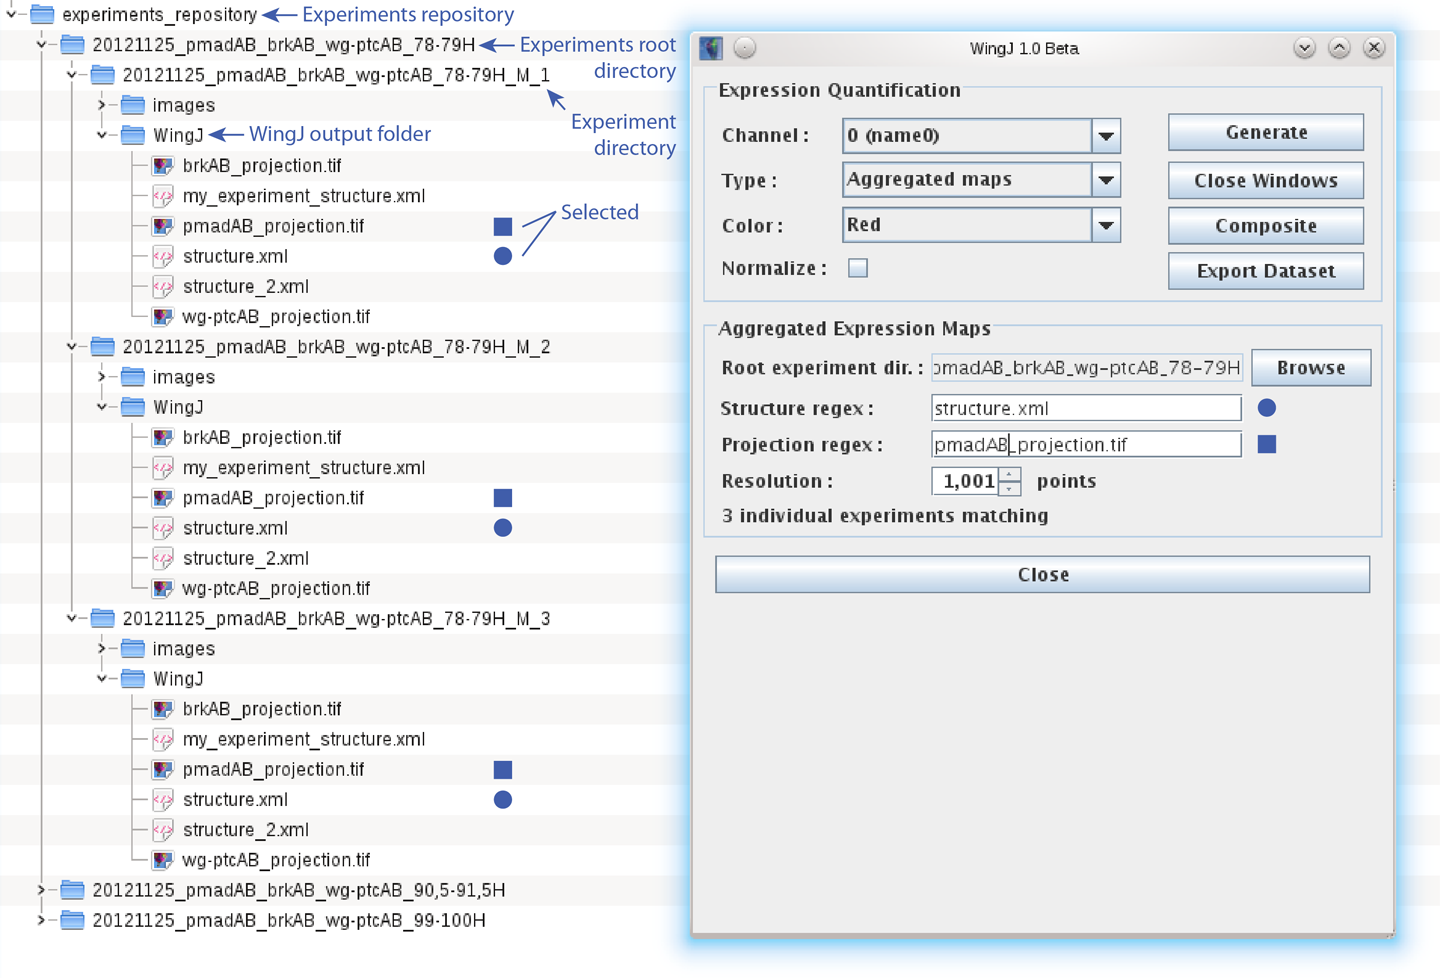
\includegraphics[scale=1.2]{images/regex2_cropped_1440.png}
\caption{\textbf{Selection of structure and expression models using regular expressions.} The specified regular expressions allow to uniquely identify the structure model and the image projection containing in each experiment folder.}
\label{fig:wingj_regex2}
\end{figure}

\begin{figure}[!h]
\centering
% \includegraphics[scale=0.7]{images/wingj_expression_maps_mean_interface.jpg}
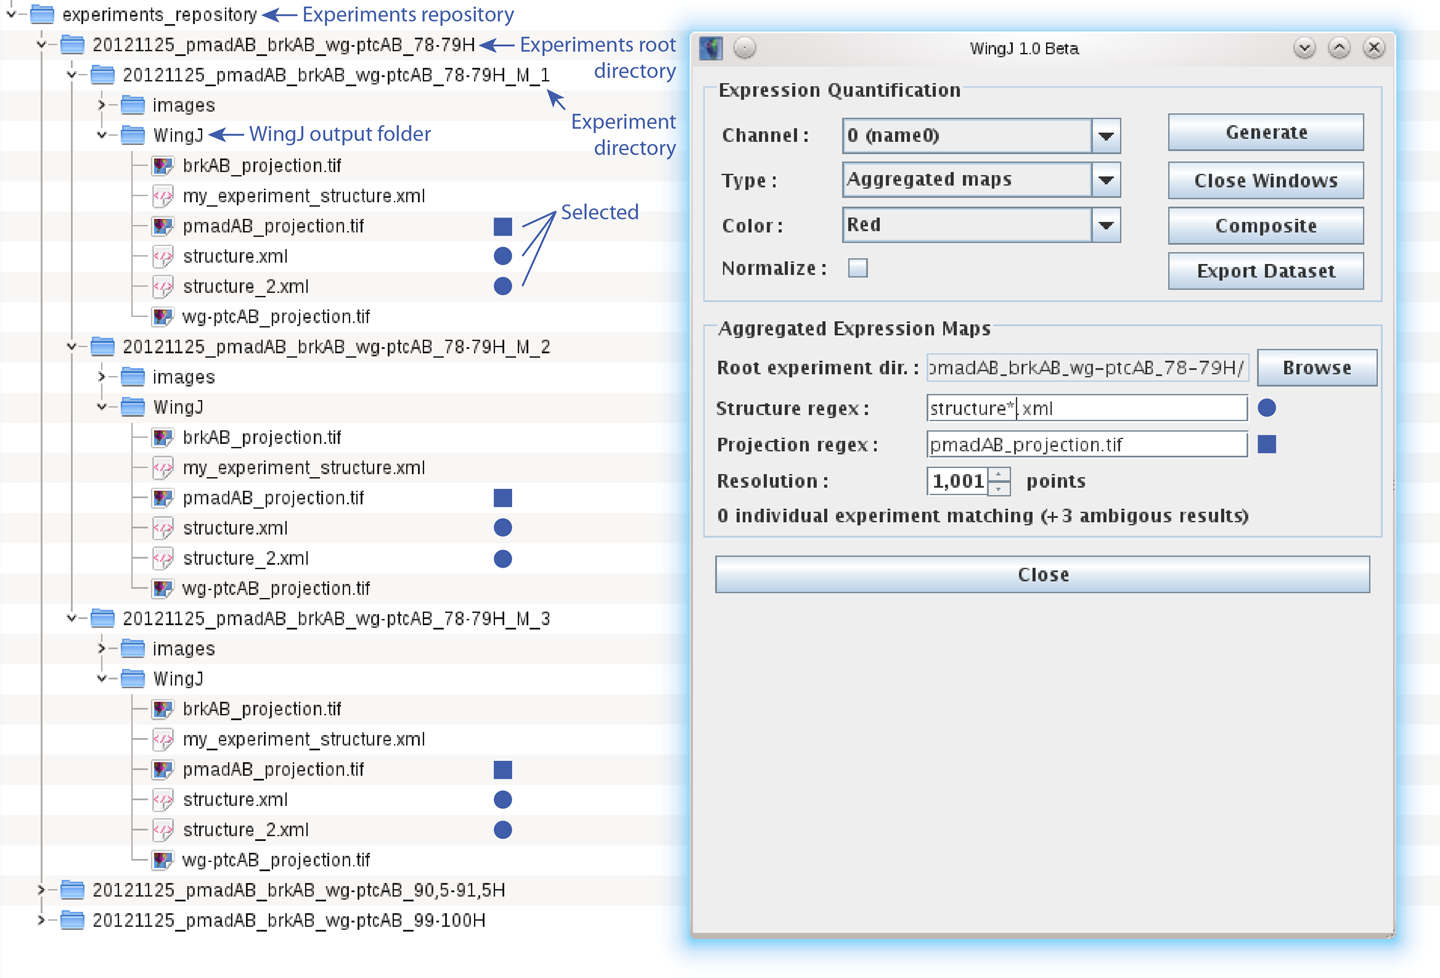
\includegraphics[scale=1.2]{images/regex3_cropped_1440.png}
\caption{\textbf{Illustration of the wildcard '*' in regular expressions.} The wildcard can be used to avoid having to enter a very long string. Here however, the wildcard leads to ambiguous results because more than one projection match the regular expression specified.}
\label{fig:wingj_regex3}
\end{figure}

\begin{figure}[!h]
\centering
% \includegraphics[scale=0.7]{images/wingj_expression_maps_mean_interface.jpg}
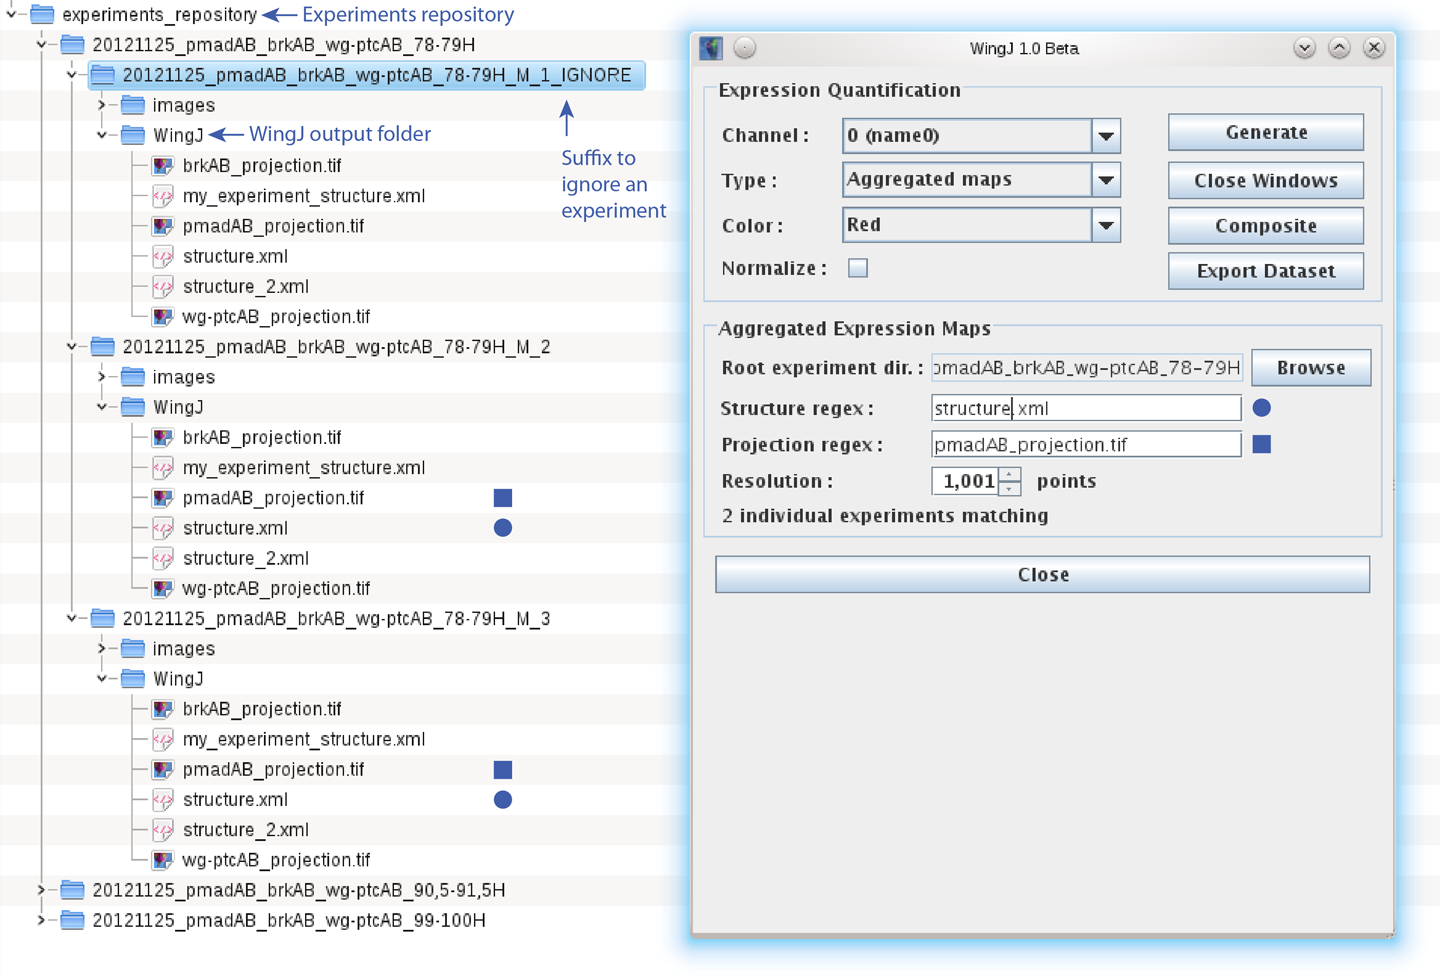
\includegraphics[scale=1.2]{images/regex4_cropped_1440.png}
\caption{\textbf{Discarding experiment folder when generating mean models.} The suffix "IGNORE" (we suggest to append "\_IGNORE") can be appended to the name of an experiment folder to tell \wingj to ignore it. This tag is also recognized by the \wingjMatlab when analyzing structure and expression datasets.}
\label{fig:wingj_regex4}
\end{figure}

% ===============================================================================
\subsection{Dataset}
Click on \textit{Export} to save the dataset to files. The files written are:

\begin{itemize}
 \item \textbf{mean\_expression\_map.xml}. The mean structure model exported in \wingj format (average structure model computed from individual structure models). Moreover, three files containing the coordinates of points describing the A/P and D/V boundaries, and the contour of the structure are saved to text files.
 \item \textbf{mean\_expression\_map\_meanPlusStd.xml}. Same as above but the contour of the structure represents the mean structure contour plus the standard deviation.
 \item \textbf{mean\_expression\_circular.tif}. The mean circular expression maps computed from many experiments. This expression map is a square image and is exported in TIFF format. The background of the image is black.
 \item \textbf{mean\_expression\_circular\_std.tif}. Same as above but representing the standard deviation of the pixel values computed when aggregating the individual circular expression maps. The image is exported in TIFF format.
 \item \textbf{mean\_expression\_circular\_mask.tif}. Binary image in TIFF format and square format that can be used as a mask for the above mean circular expression map. Pixels corresponding to the circular expression map are set to white (255), otherwise black (0).
 \item \textbf{mean\_expression\_map.tif}. The mean expression map (average expression map) wrapped on the average structure model. This expression map is then saved in TIFF format. The background of the image is black.
 \item \textbf{mean\_expression\_map\_plus.tif}. The mean expression map augmented with information about the orientation of the structure model. The image is saved in TIFF format.
 \item \textbf{mean\_expression\_map\_std.tif}. Same as above but here the circular standard deviation expression map is wrapped on the average structure model.
 \item \textbf{mean\_expression\_map\_std\_plus.tif}. Same as above but augmented with information about the orientation of the structure model. The image is saved in TIFF format.
 \item \textbf{mean\_expression\_map\_meanPlusStd.tif}. Same as the mean expression map where the contour of the mean+std structure is shown. The image is saved in TIFF format.
 \item \textbf{mean\_expression\_map\_mask.tif}. Binary image in TIFF format for the mean expression map. Pixels corresponding to the circular expression map are set to white (255), otherwise black (0).
 \item \textbf{mean\_expression\_map\_meanPlusStd\_mask.tif}. Binary image in TIFF format computed from the mean+std structure model.
\end{itemize}

% ===============================================================================
\section{Generating composite images}\label{sec:expression_composite}
The \textit{Expression panel} provides a tool to generate composite images from the stacks of confocal images imported in \wingj. Use the option \textit{Color} to assign a color to each image channels. Up to three channels can be used for generating RGB composite images. The method takes into account the index of the minimum and maximum z-slice (\sectionref{sec:structure_slice_index}) and projection method (\sectionref{sec:structure_projections}) specified for each channel from the main interface of \wingj.\\

As an example, \figureref{fig:composite} shows the composite image generated for Wg-Ptc (blue, max intensity projection), Pmad (green, mean intensity projection) and Brk (red, mean intensity projection).

\begin{figure}[!h]
\centering
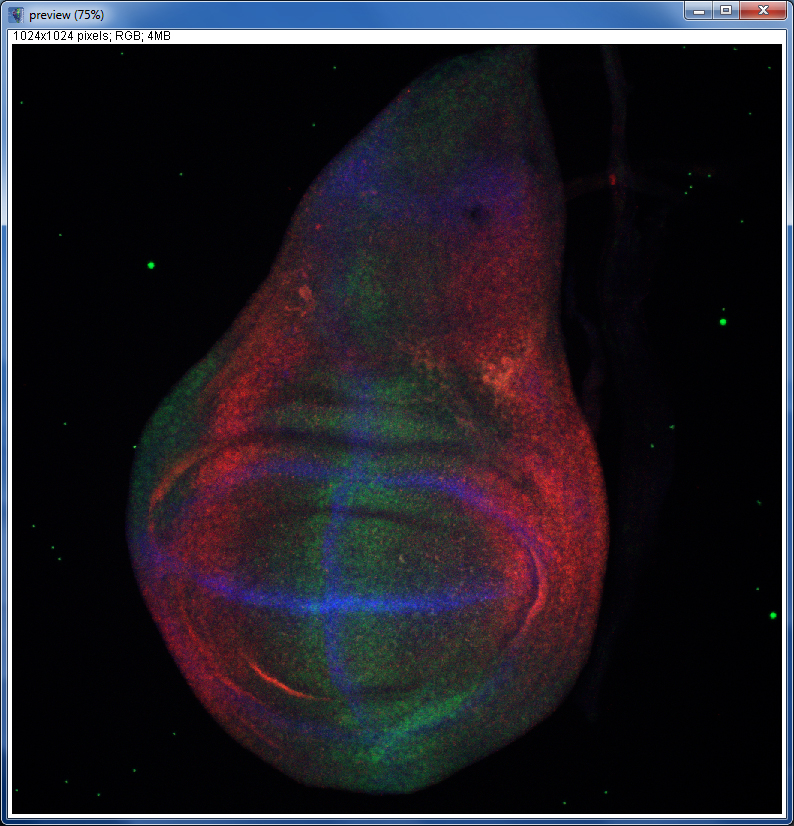
\includegraphics[scale=0.4]{images/composite.jpg}
\caption{\textbf{Composite image generated from three stacks of confocal images imported in \wingj.} The composite image supports up to three channels (RGB color space used). The method takes into account the index of the minimum and maximum z-slice and projection method specified for each channel from the main interface of \wingj. Here, the input channels are Wg-Ptc (blue, max intensity projection), Pmad (green, mean intensity projection) and Brk (red, mean intensity projection.}
\label{fig:composite}
\end{figure}

% Here we give a short description for each control:
% 
% \begin{itemize}
%  \item \textbf{Slices}\\Defines the index of the lower and upper \emph{image slice} from the loaded image stack. Both values are set to 1 if a single image is loaded. Only images between the lower and upper slice are taken into account. The other slice images are discarded.\\
% 
%  \item \textbf{Sigma}\\Standard deviation of the 1D Gaussian filter used to measure gene expression. For each spatial point of the 1D expression profile quantified, for example along the D/V boundary, pixels \emph{perpendicular} to that point and falling into the Gaussian are used to obtain an estimation of gene expression.\\
% 
%  \item \textbf{Shift}\\Gene expression is measured by default along the detected D/V or A/P boundary. If the D/V (A/P) boundary is used as reference, this parameter allows to \emph{translate} it along the trajectory of the A/P (D/V) boundary. \emph{Negative values} shift the trajectory along which the expression is measured towards the Dorsal (Anterior) side of the wing, and \emph{positive values} towards Ventral (Posterior) side.\\
% 
%  \item \textbf{Lengths}\\Each compartment boundary is decomposed into two branches: the D/V boundary is composed of the two branches/polygons D-C and C-V. The point C refers to the center of the wing pouch. The A/P boundary is composed of the branches A-C and C-P. The two fields following \emph{Lengths} show the length in $[\mu m]$ of each couple of branches.\\
% 
%  \item \textbf{Reference boundary}\\Reference boundary along which gene expression is measured.\\
% 
%  \item \textbf{Plot}\\Shows the quantified profile of gene expression and the spatial region where expression is measured. The origin of the plot corresponds to the intersection of the D/V and A/P boundaries.\\
% 
%  \item \textbf{Save Dataset}\\Save the quantified gene expression profile in TSV format. The origin of the plot corresponds to the intersection of the D/V and A/P boundaries.
% \end{itemize}
% 
% \textbf{Tip:} crop the range of the slice images to remove unwanted fluorescence, for example from the \emph{peripodial membrane} of the \textit{Drosophila} wing imaginal disc.

% \subsection{Quantification along D/V and A/P boundaries}
% 
% After having loaded the \emph{expression image}, click on the button \emph{Plot} from the main interface of WingJ. The expression is measured by default along the D/V boundary. The D/V boundary is also called \emph{AP axis}. In WingJ, \emph{AP axis} means the D/V boundary with the additional information that the boundary is running \emph{from the Anterior to the Posterior side} of the \textit{Drosophila} wing. Idem for the A/P boundary, which is also called \emph{DV axis} and running \emph{from the Dorsal to Ventral side} of the wing. Fig. \ref{fig:expression_plot} and \ref{fig:expression_plot_ap} illustrate the quantification of gene expression along the AP and DV axes, respectively.\\

% \begin{figure}[h!]
% \centering\includegraphics[width=10.4cm]{figures/expression_plot}
% \caption{Quantification of gene expression along the D/V boundary (AP axis). X-axis corresponds to the spatial axis in $[\mu m]$ with negative values for the Dorsal side of the wing. Y-axis represents the absolute fluorescence intensity (0-255), which is proportional to gene expression. A second window shows where the gene expression is measured.}
% \label{fig:expression_plot}
% \end{figure}
% 
% \begin{figure}[h!]
% \centering\includegraphics[width=10.4cm]{figures/expression_plot_ap}
% \caption{Quantification of gene expression along the A/P boundary (DV axis). X-axis corresponds to the spatial axis in $[\mu m]$ with negative values for the Anterior side of the wing. Y-axis represents the absolute fluorescence intensity (0-255), which is proportional to gene expression. A second window shows where the gene expression is measured.}
% \label{fig:expression_plot_ap}
% \end{figure}

% The first window shows the measured gene expression profile. The x-axis is the spatial axis along which the expression is measured, for instance the AP axis. The origin of the plot corresponds to the intersection of the D/V and A/P boundaries. Thus, negative spatial values correspond either to the Dorsal or Anterior sides, and positive spatial values either to Ventral or Posterior sides of the \textit{Drosophila} wing. Y-axis corresponds to the absolute fluorescence intensity, which is proportional to gene expression. Y-axis values run from 0 (black, gene not expressed) to 255 (white, maximum value of gene expression).\\
% 
% The second window shows \emph{where} the gene expression has been measured. In Fig. \ref{fig:expression_plot}, the x-axis corresponds to the AP axis and is shown as a cyan polygon. The contour of the detected \textit{Drosophila} wing pouch is also made visible. To obtain a better estimation of the gene expression compared to simply looking at a single pixel value along the x-axis, a 1D Gaussian filter is defined perpendicularly to each point of the x-axis. The standard deviation $\sigma$ of the Gaussian filter can be set via the parameter field \emph{Sigma} from the main interface of WingJ. The total width of the cyan \emph{ribbon} in Fig. \ref{fig:expression_plot} and \ref{fig:expression_plot_ap} is $6\sigma$.\\
% 
% \textbf{Tip}: title, x-axis, and y-axis labels of the gene expression plots can be edited by \emph{right-clicking} on them.
% 
% \subsection{Quantification along custom spatial trajectories}
% 
% Gene expression profiles are quantify by default along the D/V and A/P boundaries (reference boundaries). WingJ also allows to measure the expression \emph{anywhere} inside the detected \textit{Drosophila} wing pouch structure. Fig. \ref{fig:expression_shift} (Left) illustrates the case where the parameter \emph{Shift} = -40 $[\mu m]$. Because the D/V boundary has been selected has reference boundary, the trajectory where the expression is measured is translated towards the Dorsal side of the wing. A positive value would have translated it towards the Ventral side. If the reference boundary was the A/P boundary, negative and positive values for \emph{Shift} would have resulted in translations towards the Anterior and Posterior sides, respectively. In addition, the parameters \emph{Lengths} can both be set to constrain the spatial trajectory to the interior of the wing pouch, as shown in Fig. \ref{fig:expression_shift} (Right).

% \begin{figure}[h!]
% \begin{center}
% \begin{minipage}[b]{0.45\linewidth}
% \centering
% \includegraphics[width=6cm]{figures/expression_shift_m40}
% \end{minipage}
% \hspace{0.5cm}
% \begin{minipage}[b]{0.45\linewidth}
% \centering
% \includegraphics[width=6cm]{figures/expression_shift_m40_cropped}
% \end{minipage}
% \end{center}
% \caption{Quantification of gene expression along a custom trajectory. Start by selecting the reference boundary among the A/P and D/V boundaries (here the D/V boundary). (Left) The parameter \emph{Shift} is set to -40 $[\mu m]$, which results in a translation of the trajectory towards the Dorsal side of the wing. (Right) Here the total length of D/V boundary is 340 $[\mu m]$, which correponds to the sum of the branch running from the center of the pouch to the P extremity (158 $[\mu m]$) and the branch running form the center of the pouch to the A extremity (156 $[\mu m]$). The parameters \emph{Fields} are both decreased to constrain the spatial trajectory to the interior of \textit{Drosophila} the wing pouch.}
% \label{fig:expression_shift}
% \end{figure}

% \subsection{Exporting gene expression profiles}
% 
% Gene expression profiles can be saved in TSV (tab-separated values) format from the interface of WingJ. The exported files contain two columns. The first column represents the \emph{spatial trajectory} with values in $[\mu m]$ running form negative to positive. The origin corresponds to the intersection of the D/V and A/P boundaries. The second column represents the absolute fluorescence intensity measured, with values ranging from 0 (black, gene not expressed) to 255 (white, maximum value of gene expression). The following listing shows the typical content of a TSV files generated by WingJ.
% 
% \begin{verbatim}
% -136.61406382988602	67.37520586757287
% -135.27325810197462	107.69211350177174
% -134.42525810197463	95.59399280635778
% ...
% -3.460805727911321	206.51202211840592
% -2.1199999999999193	222.03970490558524
% -1.271999999999906	224.67985139008485
% 8.526512829121202E-14	228.8034195770027
% 1.2720000000000766	231.98124871878974
% 2.544000000000068	230.4245750883235
% ...
% 139.22786231553235	19.700948488654607
% 140.42711541642475	20.036271711609203
% \end{verbatim}
